%----------------------------------------------------------------------------
\chapter{Követelményspecifikáció}\label{sect:kovspec}
%----------------------------------------------------------------------------
A feladatunk egy tőzsdei kereskedési rendszer megvalósítása egy fejlett alkalmazás keretrendszer és többrétegű architektúra segítségével. A fejezet elején \sectref{defs} definiáljuk az alkalmazás fejlesztése közben előkerülő fogalmakat, majd bemutatjuk a különböző felhasználó típusokat akik használhatják a rendszert.
A \sectref{use_case} fejezetben bemutatjuk a legfontosabb felhasználói eseteket, majd a \sectref{all_use_case} fejezetben felsoroljuk az összes funkciót amit a rendszer támogatni fog. A \sectref{ui_design} részben felvázoljuk hogyan fognak kinézni a legfontosabb funkciók a képernyőn, illetve milyen lesz a képernyő elrendezése.
A fejezet végén röviden kitérünk az alkalmazás használata során felmerülő biztonsági problémákra \sectref{security}, majd bemutatjuk a tervezett architektúrát \sectref{designed_architecture}.

%,,,,,,,,,,,,,,,,,,,,,,,,,,,,,,,,,,,,,,,,,,,,,,,,,,,,,,,,,,,,,,,,,,,,,,,,,,,,
\section{Definíciók}\label{sect:defs}
%,,,,,,,,,,,,,,,,,,,,,,,,,,,,,,,,,,,,,,,,,,,,,,,,,,,,,,,,,,,,,,,,,,,,,,,,,,,,

\subsection{Felhasználó}
A rendszert felhasználók használják akiknek authentikálniuk kell magukat a rendszerbe való belépéshez. Minden felhasználóról tároljuk a nevét, a jogosultági körét és a jelszavát. Három féle felhasználót különböztetünk meg: \emph{ügyfél}, \emph{bróker}, \emph{adminisztrátor}.
\newline \underline{Adatok}: email cím, előnév, utónév, jelszó, szerepkör
\newline \underline{Megkötések}: kötelező a név, jelszó, email cím, szerepkör megadása

\subsection{Ügyfél}
Az ügyfél egy felhasználó. Miután beléptek a rendszerbe látják az árfolyamok aktuális alakulását és \emph{megbízásokat} köthetnek (vétel-eladás) bizonyos \emph{tőzsdei instrumentumra}. Lehetőségük van több \emph{számlát} fenntartani és mindegyikről külön \emph{megbízásokat} kötni, de legalább egy \emph{számlájuknak} kötelező lenni. Listázhatja éppen futó \emph{megbízásait} vagy nyomon követheti aktuális \emph{ügyleteit}.
\newline \underline{Megkötések}: legalább egy számlája van
\newline \underline{Adatok}: számlák, megbízások, ügyletek

\subsection{Tőzsdei instrumentum}
A tőzsdén jegyzett és kereskedhető eszközök, amikkel az ügyfelek kereskedhetnek a rendszer segítségével, eladási vagy vételi \emph{megbízásokat} köthetnek rájuk. Az áruk folyamatosan valós időben megjelenik az ügyfél előtt.
\newline \underline{Adatok}: aktuális ár

\subsection{Számla}
Minden ügyfélnek van legalább egy számlája, de akár több is. A számlának van egy \emph{egyenlege} ami az aktuálisian felhasználható pénz mennyisége. Minden számlához tartoznhatnak \emph{megbízások}, \emph{ügyletek}. Egy vételi megbízás indításakor a számláról lekerül a fedezet, majd ha az ügylet záros határidőn belül nem jön létre, a pénz visszakerül, egyébként végleg lekerül. Ha egy eladás ügylet létrejön az áru ára rákerül a az adott számlára (ahonnan az véve lett).
\newline \underline{Megkötések}: nem létezhet ügyfél nélkül
\newline \underline{Adatok}: egyenleg, megbízások, ügyletek

\subsection{Egyenleg}
A számlán aktuálisan található \emph{pénz összege}. Maximum ekkora értékű megbízás indítható az adott számláról.
\newline \underline{Adatok}: pénz összeg
\newline \underline{Megkotesek}: minden számlához tartozik

\subsection{Megbízás}
Egy megbízás lehet \emph{eladás} vagy \emph{vétel} egy adott tőzsdei instrumentumra, amelyet az ügyfél kezdeményez adott áron, adott mennyiségre. Ha két ellentétes tipusú és ugyanolyan áru megbízás találkozik akkor létrejön egy \emph{ügylet}. A mennyiségek osztódhatnak több ügyletre.
\newline \underline{Megkötések}: számlához tartozik (így ügyfélhez is)
\newline \underline{Adatok}: számla, instrumentum neve, mennyiség, ár, típus(vétel/eladás), kezdeményezés dátuma

\subsection{Ügylet}
Ha két ellentétes tipusú \emph{megbízás} történik egy idő intervallumban létrejön egy ügylet és a tőzsdei instrumentum gazdát cserélnek. A vevő számlájáról végleg lekerül a pénz, míg az eladóéra rákerül.
\newline \underline{Adatok}: két megbízás, mennyiség, dátum amikor létrejött
\newline \underline{Megkötések}: két ellentétes tipusú ügylet kell hozzá

\subsection{Bróker}
A bróker egy felhasználó. Megnézheti egy adott \emph{ügyfél} \emph{számláit} élő vagy inaktív \emph{megbízásait}, \emph{ügyleteit}.

\subsection{Adminisztrátor}
Az ügyfelek, brókerek \emph{regisztrációját} végzi a rendszerbe. Akár \emph{deaktiválhatja} is felhasználókat, ő a rendszer ura.


%,,,,,,,,,,,,,,,,,,,,,,,,,,,,,,,,,,,,,,,,,,,,,,,,,,,,,,,,,,,,,,,,,,,,,,,,,,,,
\section{Felhasználói szerepkörök}\label{sect:roles}
%,,,,,,,,,,,,,,,,,,,,,,,,,,,,,,,,,,,,,,,,,,,,,,,,,,,,,,,,,,,,,,,,,,,,,,,,,,,,

Mint fentebb már említettük három különböző felhasználói szerepkört különböztetünk meg a rendszerben.

\subsection{Ügyfél}
Miután belép látja az aktuális árfolyamokat és eladási vagy vételi megbízást indíthat akár azonnal. Listázni tudja a megbízásait, visszavonni, módosítani, látja a régebbi ügyleteit. Szintén listázni tudja a számláit, látja az aktuális egyenlegét, új számlákat tud létrehozni, tud utalni pénzt a számlájára.

\subsection{Bróker}
Látja az összes ügyfél adatait, megbízásait, ügyleteit, számláit.

\subsection{Adminisztrátor}
Rendelkezik ugyanazokkal a szerepekkel, mint egy bróker, de képes regisztrálni brókert, ügyfelet vagy akár törölheti is őket a rendserből.

%,,,,,,,,,,,,,,,,,,,,,,,,,,,,,,,,,,,,,,,,,,,,,,,,,,,,,,,,,,,,,,,,,,,,,,,,,,,,
\section{Leggyakoribb felhasználói esetek}\label{sect:use_case}

\subsection{Regisztráció kérelme}
A felhasználó egy felületen a szükséges adatok bevitelével regisztrációt kérvényez ami az adminisztrátorhoz kerül felülvizsgálatra. Az adminisztrátor engedélyezheti, elvetheti a kérelmet.
\newline \underline{Szerepkör}: Ügyfél, Adminisztrátor, Bróker

\subsection{Megbízás adása}
A felhasználó kitölt egy megbízási formulát, melyhez megadja a szükséges adatokat(instrumentum, mennyiség, eladás/vétel, ár), majd ezt beregisztrálja a rendszerbe.
\newline \underline{Szerepkör}: Ügyfél

\subsection{Megbízás visszavonása}
A felhasználó eltávolít egy megbízást.
\newline \underline{Szerepkör}: Ügyfél

\subsection{Ügyfél megbízásainak listázása}
A felhasználó kilistázza egy lapozható listában az összes aktív/inaktív megbízását.
\newline \underline{Szerepkör}: Bróker, Ügyfél (csak a sajátját)

\subsection{Ügyfél ügyleteinek historikus listázása}
A felhasználó kilistázza egy lapozható listában az összes ügyletet, ami az ügyfél megbízásai által jött létre. Az ügyleteket szűrhetjük aszerint, hogy eladók vagy vásárló az ügyfél.
\newline \underline{Szerepkör}: Bróker, Ügyfél (csak a sajátját)

%,,,,,,,,,,,,,,,,,,,,,,,,,,,,,,,,,,,,,,,,,,,,,,,,,,,,,,,,,,,,,,,,,,,,,,,,,,,,
\section{Funkciók}\label{sect:all_use_case}
%,,,,,,,,,,,,,,,,,,,,,,,,,,,,,,,,,,,,,,,,,,,,,,,,,,,,,,,,,,,,,,,,,,,,,,,,,,,,

\subsection{Regisztráció kérelme}
A felhasználó egy felületen a szükséges adatok bevitelével regisztrációt kérvényez
\newline \underline{Szerepkör}: Ügyfél, Adminisztrátor, Bróker

\subsection{Felhasználó regisztrációja}
A felhasználó a beérkezett regisztrációs kérelmet feldolgozza és létrehoz egy új felhasználót, a role alapvetően ügyfél típusú lesz
\newline \underline{Szerepkör}: Adminisztrátor

\subsection{Felhasználó kinevezése}
Az felhasználó kinevezhet egy ügyfelet brókernek vagy adminisztrátornak
\newline \underline{Szerepkör}: Adminisztrátor

\subsection{Felhasználó deaktiválása}
A felhasználó eltávolíthat egy felhasználót és annak összes bejegyzését a rendszerből
\newline \underline{Szerepkör}: Adminisztrátor

\subsection{Ügyfél számla létrehozása}
Az felhasználó az adott ügyfél számára létrehoz egy számlát
\newline \underline{Szerepkör}: Adminisztrátor

\subsection{Ügyfél számla módosítása}
A felhasználó módosítja az ügyfélhez tartozó számlát
\newline \underline{Szerepkör}: Adminisztrátor

\subsection{Ügyfél számla törlése}
A felhasználó eltávolít egy ügyfél számlát
\newline \underline{Szerepkör}: Adminisztrátor

\subsection{Megbízás adása}
 A felhasználó kitölt egy megbízási formulát, melyhez megadja a szükséges adatokat, majd ezt beregisztrálja a rendszerbe.
\newline \underline{Szerepkör}: Ügyfél

\subsection{Megbízás módosítása}
A felhasználó módosítja az egyik megbízást.
\newline \underline{Szerepkör}: Ügyfél

\subsection{Megbízás visszavonása}
A felhasználó eltávolít egy megbízást.
\newline \underline{Szerepkör}: Ügyfél

\subsection{Ügyfél ügyleteinek historikus listázása}
A felhasználó kilistázza egy lapozható listában az összes ügyletet, ami az ügyfél megbízásai által jött létre. Az ügyleteket szűrhetjük aszerint, hogy eladók vagy vásárló az ügyfél.
\newline \underline{Szerepkör}: Bróker, Ügyfél (csak a sajátját)

\subsection{Ügyfél számláinak megtekintése}
A felhasználó lekéri egy adott ügyfél összes számlájának listáját.
\newline \underline{Szerepkör}: Bróker, Ügyfél (csak a sajátját)

\subsection{Ügyfél számlaegyenlegének megtekintése}
A bróker lekéri egy adott ügyfél adott számlájának egyenlegét.
\newline \underline{Szerepkör}: Bróker, Ügyfél (csak a sajátját)

\subsection{Ügyfél élő megbízásainak megtekintése}
A bróker lekéri egy adott ügyfél élő megbízásait.
\newline \underline{Szerepkör}: Bróker, Ügyfél (csak a sajátját)

\subsection{Ügyfél inaktív megbízásainak megtekintése}
A bróker lekéri egy adott ügyfél inaktív megbízásait.
\newline \underline{Szerepkör}: Bróker, Ügyfél (csak a sajátját)

\newpage
%,,,,,,,,,,,,,,,,,,,,,,,,,,,,,,,,,,,,,,,,,,,,,,,,,,,,,,,,,,,,,,,,,,,,,,,,,,,,
\section{Felhasználói interfész tervek}\label{sect:ui_design}
%,,,,,,,,,,,,,,,,,,,,,,,,,,,,,,,,,,,,,,,,,,,,,,,,,,,,,,,,,,,,,,,,,,,,,,,,,,,,


\subsection{Regisztráció}

\begin{figure}[!ht]
\centering
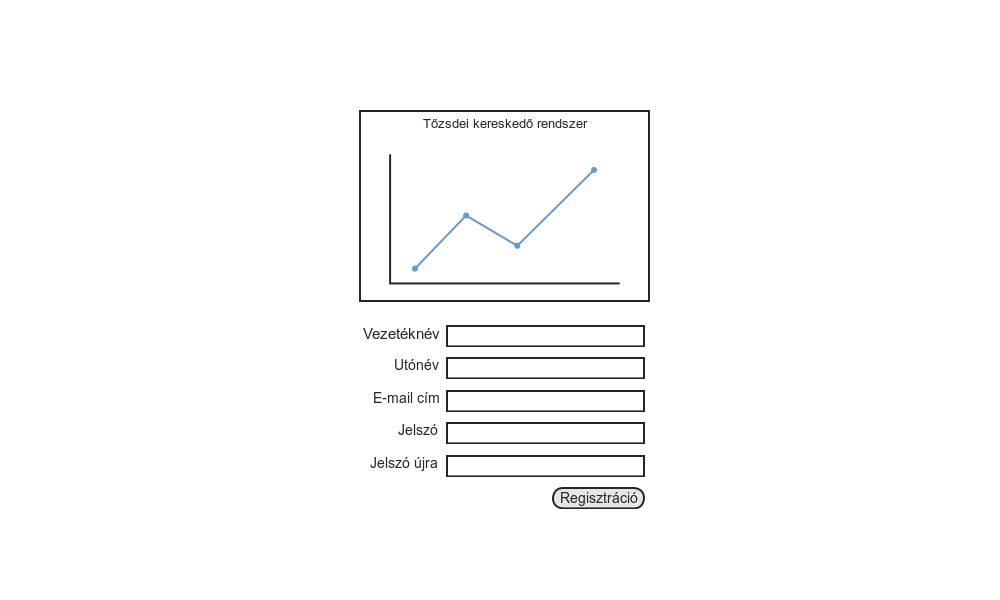
\includegraphics[width=150mm, keepaspectratio]{figures/user_1/register.png}
\caption{Regisztráció}
\label{fig:haromreteg}
\end{figure}

\subsection{Bejelentkezés}

\begin{figure}[!ht]
\centering
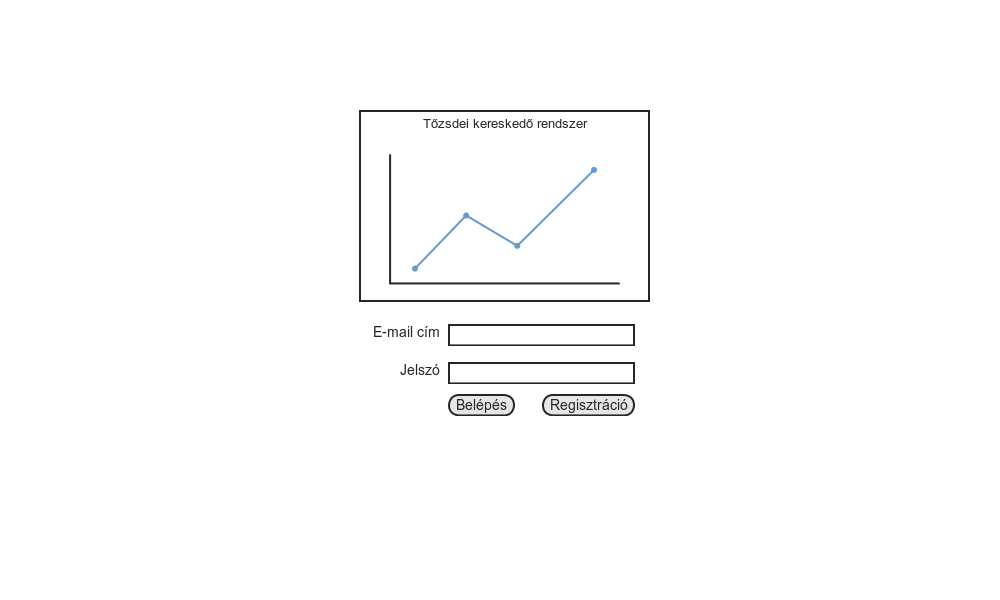
\includegraphics[width=150mm, keepaspectratio]{figures/user_1/login.png}
\caption{Bejelentkezés}
\label{fig:haromreteg}
\end{figure}

\subsection{Felhasználók menedzselése}

Az adminisztrátor ezen az oldalon tudja karbantartani a felhasználókat.

\begin{figure}[!ht]
\centering
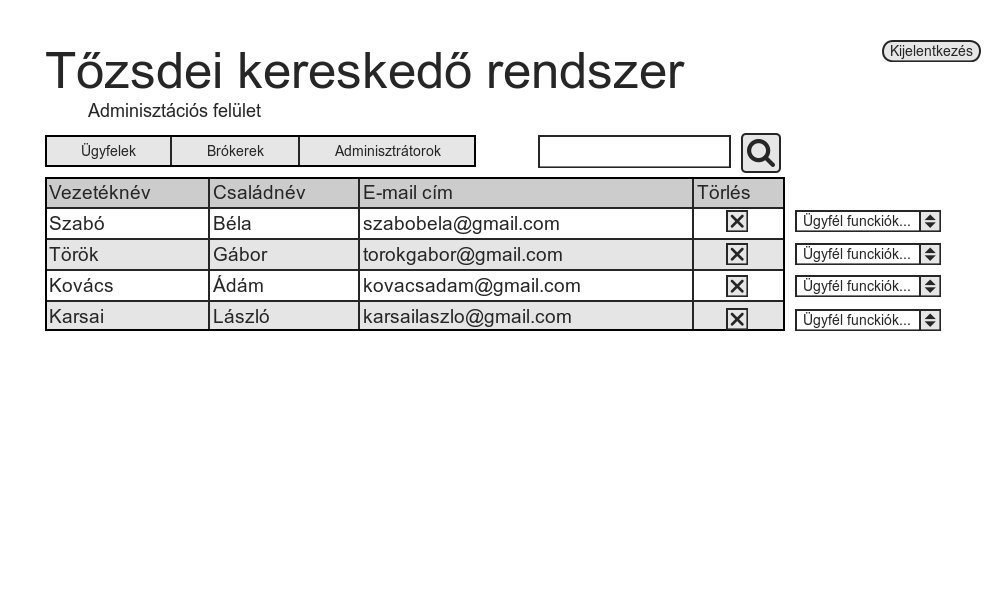
\includegraphics[width=150mm, keepaspectratio]{figures/user_1/admin_users.png}
\caption{Felhasználók menedzselése}
\label{fig:haromreteg}
\end{figure}

\subsection{Ügyfél kezdőlapja}

\begin{figure}[!ht]
\centering
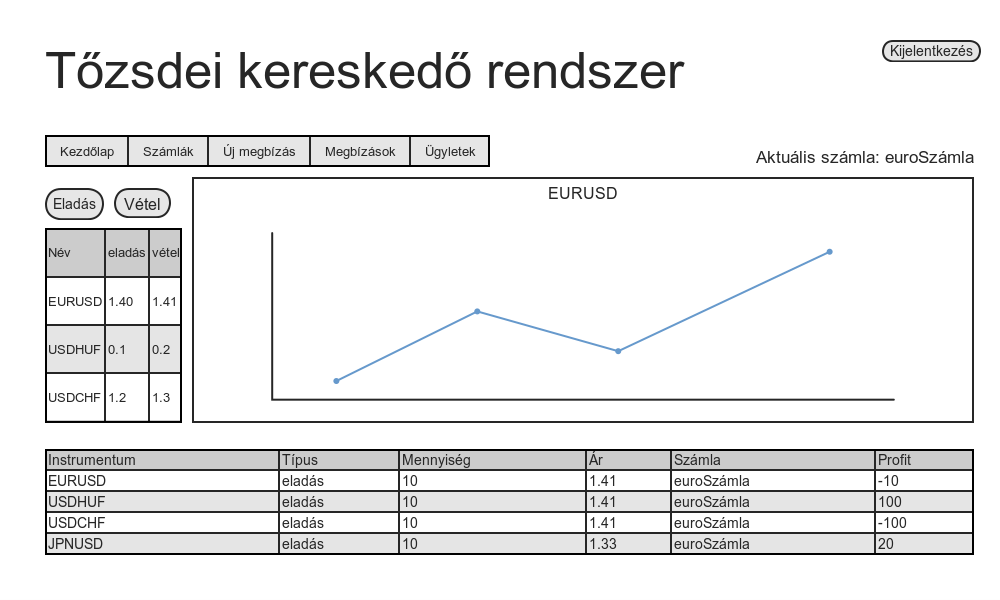
\includegraphics[width=150mm, keepaspectratio]{figures/user_1/Home.png}
\caption{Ügyfél kezdőlapja}
\label{fig:haromreteg}
\end{figure}

\subsection{Ügyfél számlái}

\begin{figure}[!ht]
\centering
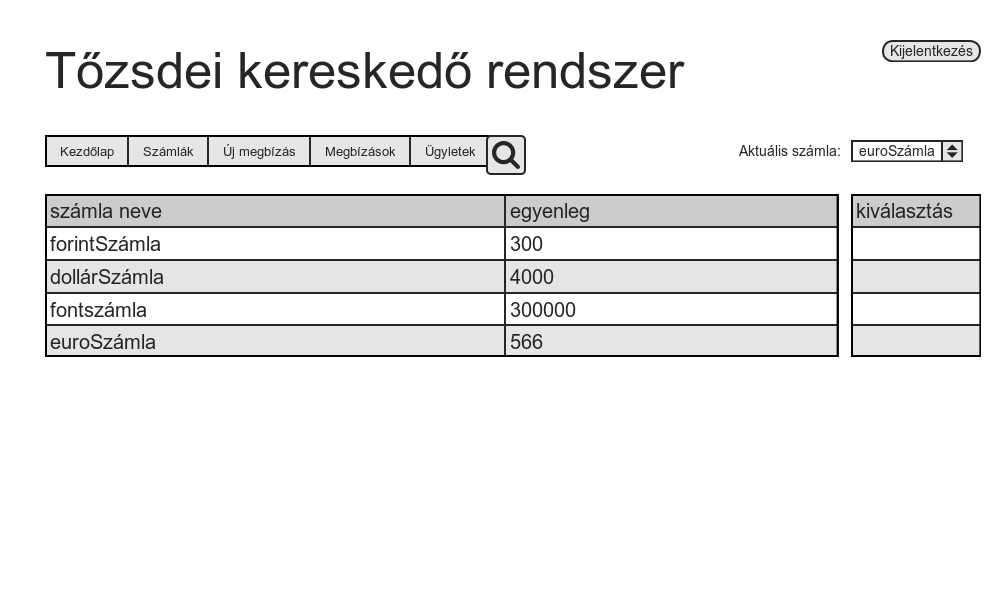
\includegraphics[width=150mm, keepaspectratio]{figures/user_1/bills.png}
\caption{Ügyfél számlái}
\label{fig:haromreteg}
\end{figure}

\subsection{Ügyfél megbízásai}
A bróker is egy hasonló oldalt lát az ügyfelek megbízásairól.

\begin{figure}[!ht]
\centering
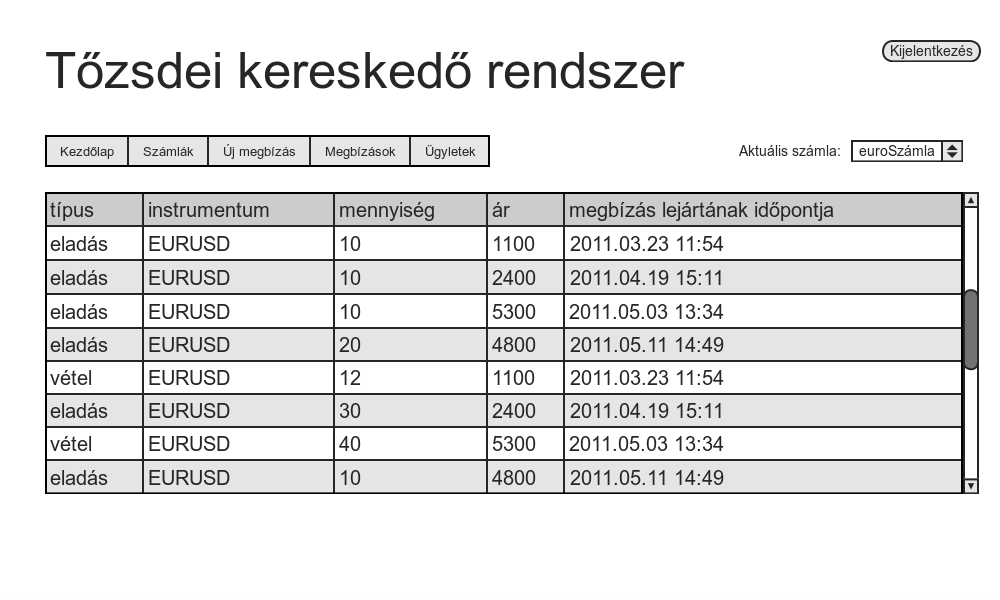
\includegraphics[width=150mm, keepaspectratio]{figures/user_1/megbizasok.png}
\caption{Ügyfél megbízásai}
\label{fig:haromreteg}
\end{figure}


\subsection{Ügyfél ügyletei}
A bróker is egy hasonló oldalt lát az ügyfelek ügyleteiről.

\begin{figure}[!ht]
\centering
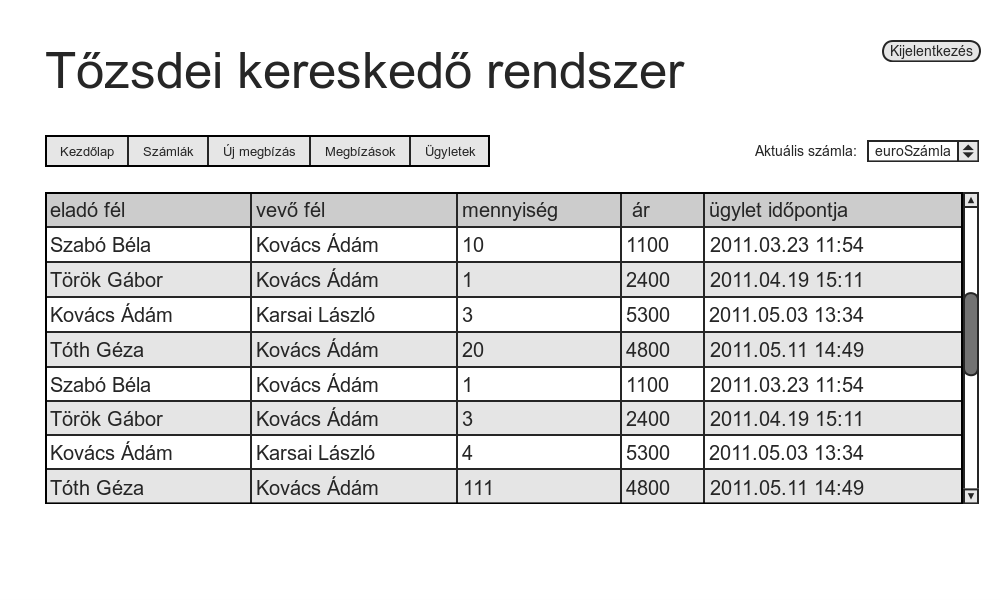
\includegraphics[width=150mm, keepaspectratio]{figures/user_1/ugyletek.png}
\caption{Ügyfél ügyletei}
\label{fig:haromreteg}
\end{figure}

\subsection{Új megbízás}

\begin{figure}[!ht]
\centering
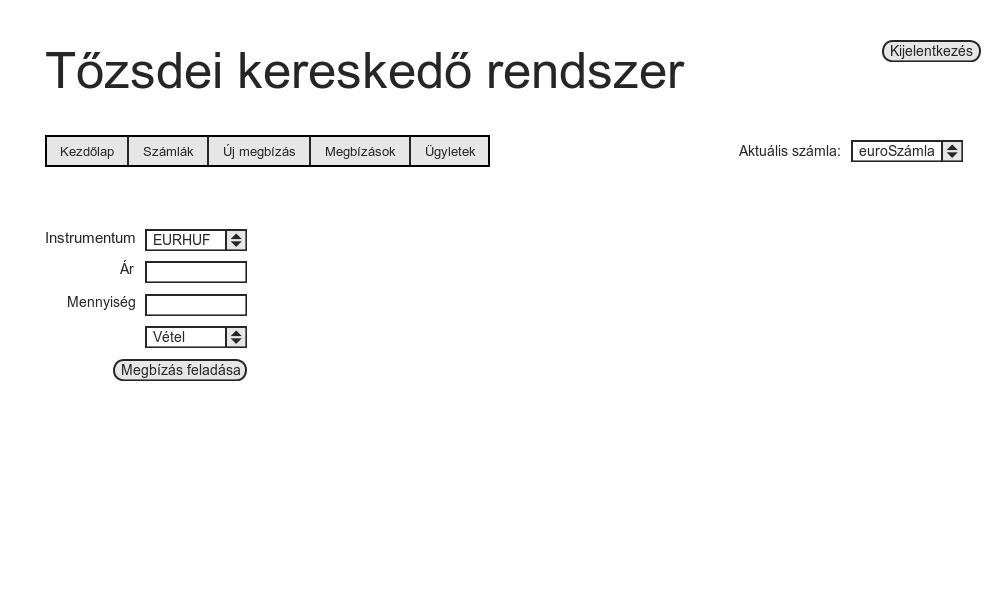
\includegraphics[width=150mm, keepaspectratio]{figures/user_1/uj_megbizas.png}
\caption{Új megbízás}
\label{fig:haromreteg}
\end{figure}

%,,,,,,,,,,,,,,,,,,,,,,,,,,,,,,,,,,,,,,,,,,,,,,,,,,,,,,,,,,,,,,,,,,,,,,,,,,,,
\section{Biztonsági követelmények}\label{sect:security}
%,,,,,,,,,,,,,,,,,,,,,,,,,,,,,,,,,,,,,,,,,,,,,,,,,,,,,,,,,,,,,,,,,,,,,,,,,,,,

\subsection{Authentikáció}
Biztonsági szempontból a legfontosabb, hogy illetéktelen személyek ne tudjanak belépni mások felhasználói fiókjába, így számukra kedvezőtlen megbízásokat indítani vagy a számlájukról pénzt lopni. Természetesen az adminisztrátori szerepkörben lévő felhasználó védelme a legfontosabb, így ott érdemes akár valamilyen fizikai (token kulcs) authentikáció használata. Mivel a rendszer nagyon sok pénzt kezelhet, így ilyen fizikai kulcsot akár minden felhasználó kaphatna a végleges rendszerben.

\subsection{Authorizáció}
A felhasználói szerepeknek élesen, pontosan el kell különülniük és implementálás után az egyes jogokat megfelelően ki kell tesztelni, így megakadályozható, hogy egy felhasználó egy másik felhasználó számlájához hozzáférhessen, esetleg megbízásokat indítson onnan vagy egyszerűen csak olyan adatokhoz jusson hozzá ami nem az ő tulajdona.

\subsection{Beviteli mezők védelme}
Természetesen a különböző beviteli mezőket védeni kell, mind SQL Injection , mind XSS ellen, így megakadályozva, hogy illetéktelen kód fusson az adatbázison vagy a kliens böngészőjében.  A kirívóan magas (a felhasználó számlájához képest) összegű megbízásokra érdemes külön visszaigazolást kérni, így elkerülhetők figyelmetlenségből, elgépelésből adódó nagyobb veszteségek.

\subsection{Biztonságos kommunikáció}
Annak érdekében, hogy egy harmadik fél ne halgathassa le a szerver-böngésző kommunikációt érdemes titkosított kapcsolatot alkalmazni, így megakadályohatjuk mind, hogy harmadik félhez illetéktelen adatok kerüljenek ki, mind, hogy egy harmadik fél a kommunikáció közepébe álljon és hamis információkat adjon a felhasználónak vagy a szervernek (pl: magasabb összzegű megbízás a felhasználó tudta nélkül).
A rendszernek rendelkeznie kell egy hivatalos harmadik fél által kiadott tanusítvánnyal ami biztosítja a felhasználót, hogy a biztonságos hálózati kommunikáció során nem egy hamis renszerrel kommunikál, hanem a valódival.

%,,,,,,,,,,,,,,,,,,,,,,,,,,,,,,,,,,,,,,,,,,,,,,,,,,,,,,,,,,,,,,,,,,,,,,,,,,,,
\section{Tervezett architektúra}\label{sect:designed_architecture}
%,,,,,,,,,,,,,,,,,,,,,,,,,,,,,,,,,,,,,,,,,,,,,,,,,,,,,,,,,,,,,,,,,,,,,,,,,,,,

A rendszert egy három rétegű architektúrában valósítjuk meg. A megjelenítést a felhasználó böngészőjében (kliens oldaon) végezzük, az üzleti logikát (megbízások, ügyletek kezelése) egy dedikált szerveren, míg az adatokat egy adatbázis rétegben tároljuk.
Az alkalmazás egy webalkalmazás lesz, a Ruby on Rails keretrendszer lesz az alapja, így a működése platformtól független lesz. 

Az alkalmazás frontendje és üzleti logikája mögött egy SQL (MySQL vagy PostgreSQL) adatbázis fog futni.

Az adatbázisban tároljuk a felhasználók rekordjait, az ügyfelek számláit és az ezekhez tartozó megbízások és ügyletek rekordjait. Új felhasználó regisztrációjakor, új számla létrehozásakor, egy megbízás feladásakor vagy egy ügylet megkötésekor egy új bejegyzés jön létre az adatbázisban, ezeket különböző felületeken a felhasználók listázzák, egyes mezőket szerkeszthetnek, felülírhatnak vagy akár törölhetnek is. A különböző entitások között tartalmazó kapcsolatok lehetnek, melyeket figyelembe kell venni az adatbázis tervezésekor.

Az adatbázisból kiolvasott és éppen használatban lévő adatokat a memóriában tároljuk, mint amilyen az aktuálisan belépett felhasználó adatai vagy az aktuálisan kiválasztott számlához tartozó információ. Ezekkel az adatokkal folyamatosan dolgozunk, így megéri őket a memóriában tartani, adatbázis hívást csak entitások listázása, új entitás létrehozása, módosítása vagy törlése esetén hívunk, módosító műveleteknél a memóriában és az adatbázisban tárolt adatok szinkronitásáról gondoskodunk.

A részvények aktuális árfolyamát a Google Finance API fogja nyújtani JSON formátumban, ezt az adatot nem szükséges az adatbázisba kimenteni, hiszen folyamatosan változik, a web service által visszaadott értékek érvényességi idejük alatt a memóriában lesznek tárolva, innen kérdezheti őket a webalkalmazás. A memóriában tárolt értékek periodikusan frissítve lesznek.


\begin{figure}[!ht]
\centering
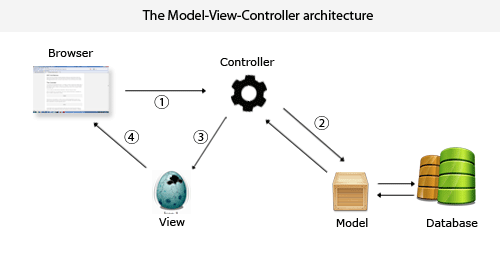
\includegraphics[width=150mm, keepaspectratio]{figures/arch.png}
\caption{Architektúra}
\label{fig:haromreteg}
\end{figure}